% Document class, paper size, base font size
\documentclass[a4paper, 12pt]{article}

% Bibliography and List of Figures in table of contents
\usepackage[nottoc,notlot]{tocbibind}

% Encoding
\usepackage[utf8]{inputenc}
\usepackage[T1]{fontenc}

% Prevent indentation of beginning of paragraphs
\setlength{\parindent}{0em}

% Space between paragraphs
\parskip 0.5em

% Farben
\usepackage[dvipsnames]{xcolor}

% include PDFs
\usepackage{pdfpages}

% For Check-List
\usepackage{enumitem}
\usepackage{amssymb,wasysym}
\usepackage{graphicx}
\usepackage{enumerate}
\newlist{todolist}{itemize}{2}
\setlist[todolist]{label=$\square$}

% Title, authors and date
\title{Software Engineering - Analysis\\
Project: E-Scooter Rental Service}

% For sources in captions
\usepackage{caption}
\captionsetup{justification=raggedright}
\newcommand{\source}[1]{\caption*{Source: {#1}}}
% \newcommand{\source}[1]{\caption*{\hfill Source: {#1}}}

\author{
    Kendra Birringer (1229372)\\
    Nader Cacace (1208115)\\
    Steffen Hanzlik (1207417)\\
    Marco Peluso (1228849)\\
    Svetozar Stojanovic (1262287)\\
    \\
    Frankfurt University of Applied Sciences
    \\ Faculty 2
}

\date{February 15th, 2020}


% Begin actual document
\begin{document}

\maketitle
\newpage
\tableofcontents

%==============================================================================
\newpage
\section{Introduction}
In this project, we took the role of a start-up company building an E-Scooter rental business.
For analyzing this project, we were encouraged to use the agile method \emph{Scrum} \cite{scrum} as a framework.

The main objective was to develop a high-level software architecture for the E-Scooter rental business. To be able to do this we had to gain a clear understanding of the system's requirements and to build a model which fulfilled these. We used the \emph{Unified Modeling Language (UML)} \cite{uml} in conjunction with the modeling tool \emph{MagicDraw} \cite{magicdraw} to achieve this.

We also had to build user interface prototypes for relevant parts of the functionality. User interface prototypes help developers and customers "to better understand how the system will work and whether it would meet the requirements." \cite{thoma} Concerning the customer, presenting her/him the prototypes, it is very important that she/he understands that these prototypes are not the finished product but are only illustrative examples to demonstrate functionality. We used \emph{Axure RP 9} \cite{axure} to create our prototypes.

For our project, the artifacts consist of diagrams and documentation for describing the software functionality. The quality of these artifacts were ensured by a proper definition of "Done".

%==============================================================================
\newpage
\section{Definition of "Done"}
The definition of "Done" (DoD) is part of the SCRUM metrics. All members of the Scrum Team must have a shared understanding of what it means when the work is complete, to ensure transparency. \cite{scrumguide}
It is a (check-)list of items which need to be validated to consider a backlog item being “Done”. DoD is defined by the development organization to make sure that the results of multiple teams can be integrated into a releasable product. \cite{thoma1}

For our project, the result needs to match the following definition of "Done":

\begin{todolist}
\item Description of the requirement in form of a Use Case
\item Categorization of requirement (functional/non-functional,\\
      client/server)
\item Business value of the corresponding functionality
\item Effort estimation for the implementation of the requirement
\item For UI related functions: UI prototype
\item UML Diagrams 

    $\bullet$ Use case diagram
    
    $\bullet$ Activity diagram
    
    $\bullet$ Class diagram
    
    $\bullet$ Sequence diagram
    
\item Detailed documentation (e.g. table) about who worked on the item and what has been done during the sprint.
\item Overall quality of the documentation meets general industry standards.
\item The results have been reviewed and accepted by another member of the team (tester). It needs to be documented who has performed the review.
\end{todolist}
%==============================================================================
\newpage
\section{High-level Software Architecture}
As you can see in figure 1, our team decided to concentrate on analyzing the Software for the Mobile Application.

\color{red}TODO: insert right picture pls \color{black}
\begin{figure} [htbp]
  \begin{center}
    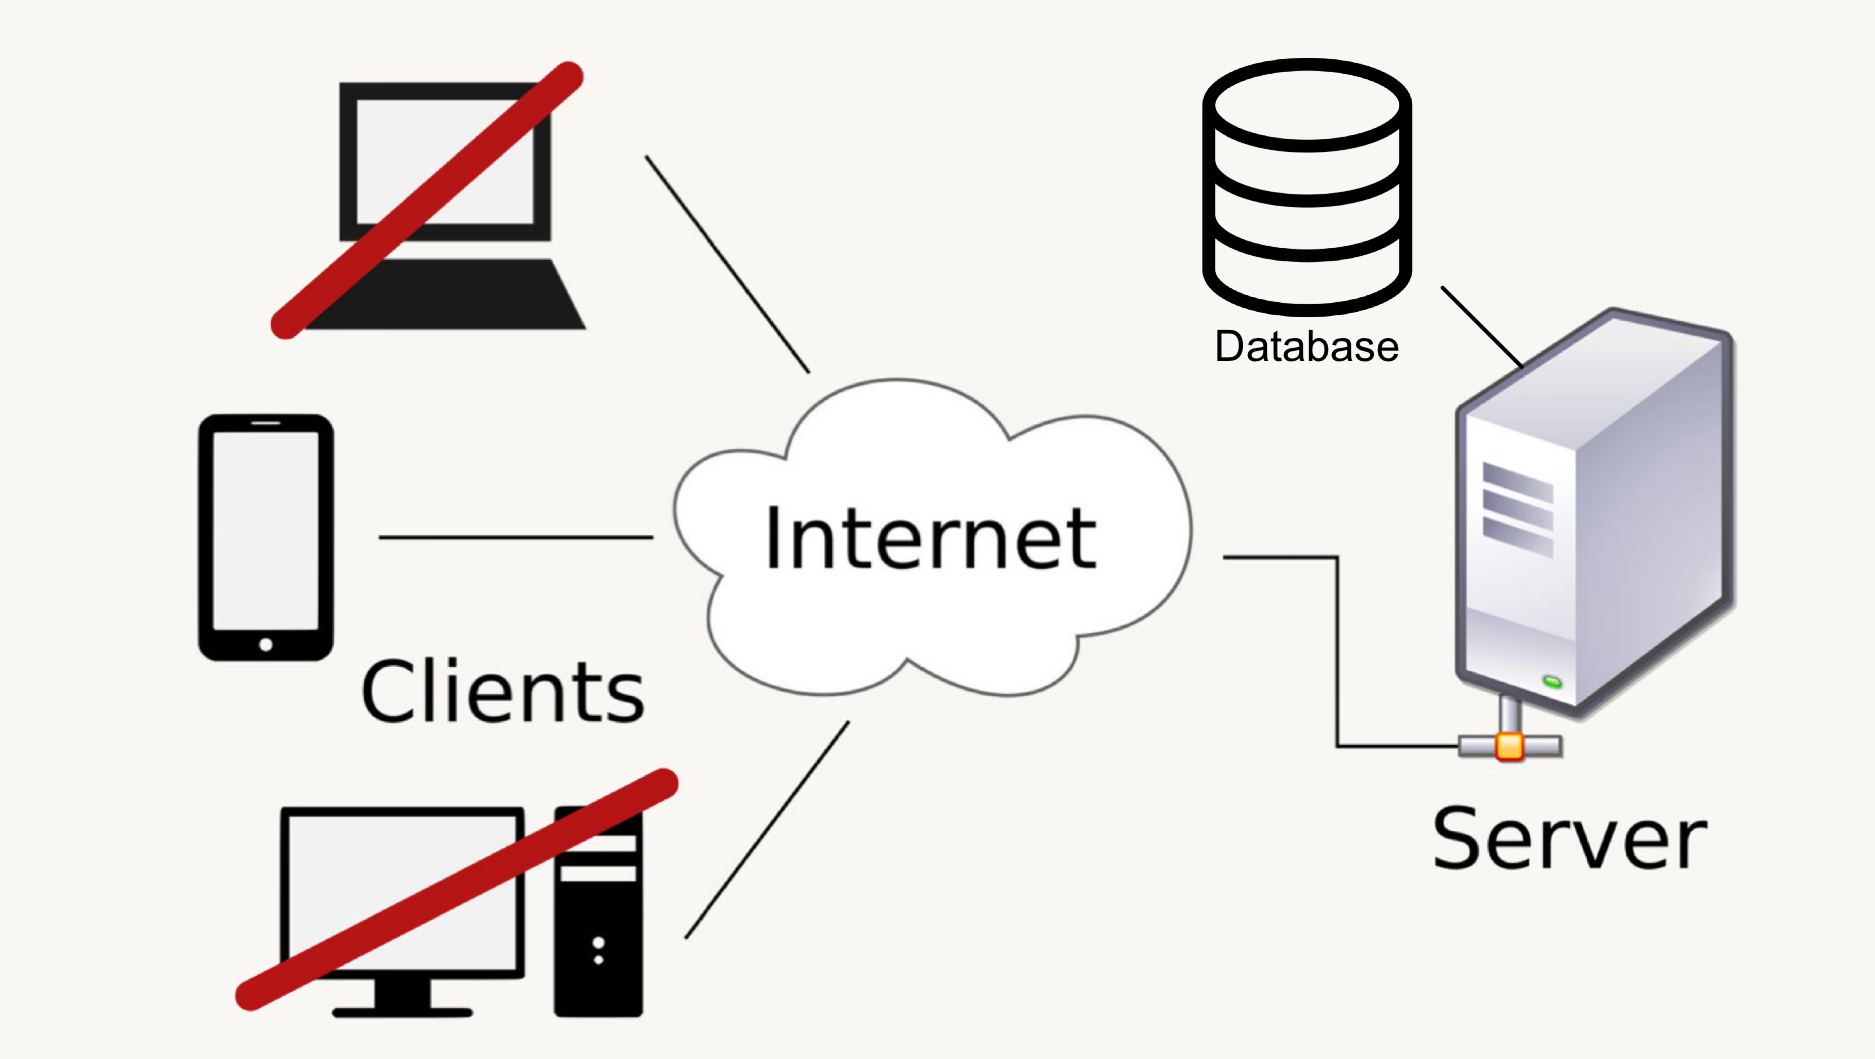
\includegraphics[scale=0.225]{images/high-level-system-architecture.jpg}
  \end{center}
  \caption{High-level software architecture}
  \source{https://commons.wikimedia.org/wiki/File:Client-server-model.svg (modified by Kendra Birringer)}
\end{figure}
%==============================================================================
\newpage
\section{Backlog Items}
Backlog items are part of a product backlog. This is an ordered list of requirements which have to be satisfied according to the DoD for the product. The purpose of a backlog item is to take a requirement description, in form of a use case description, as input and build an analysis model of our software capability as result.

We used the "Volere Requirements Specification Template" \cite{volere} also known as "Volere Snow Cards"  as a template to create a list of backlog items using Google Sheets where we collected all of our backlog items. This requirement matrix is shown in figure \ref{fig:reqmatrix}.

\color{red}TODO: FIX Requirements-Matrix as a figure to be able to reference it.
Possible workaround: convert pdf to images and insert them as figures.
\color{black}

% \begin{figure} [htbp]
\label{fig:reqmatrix}
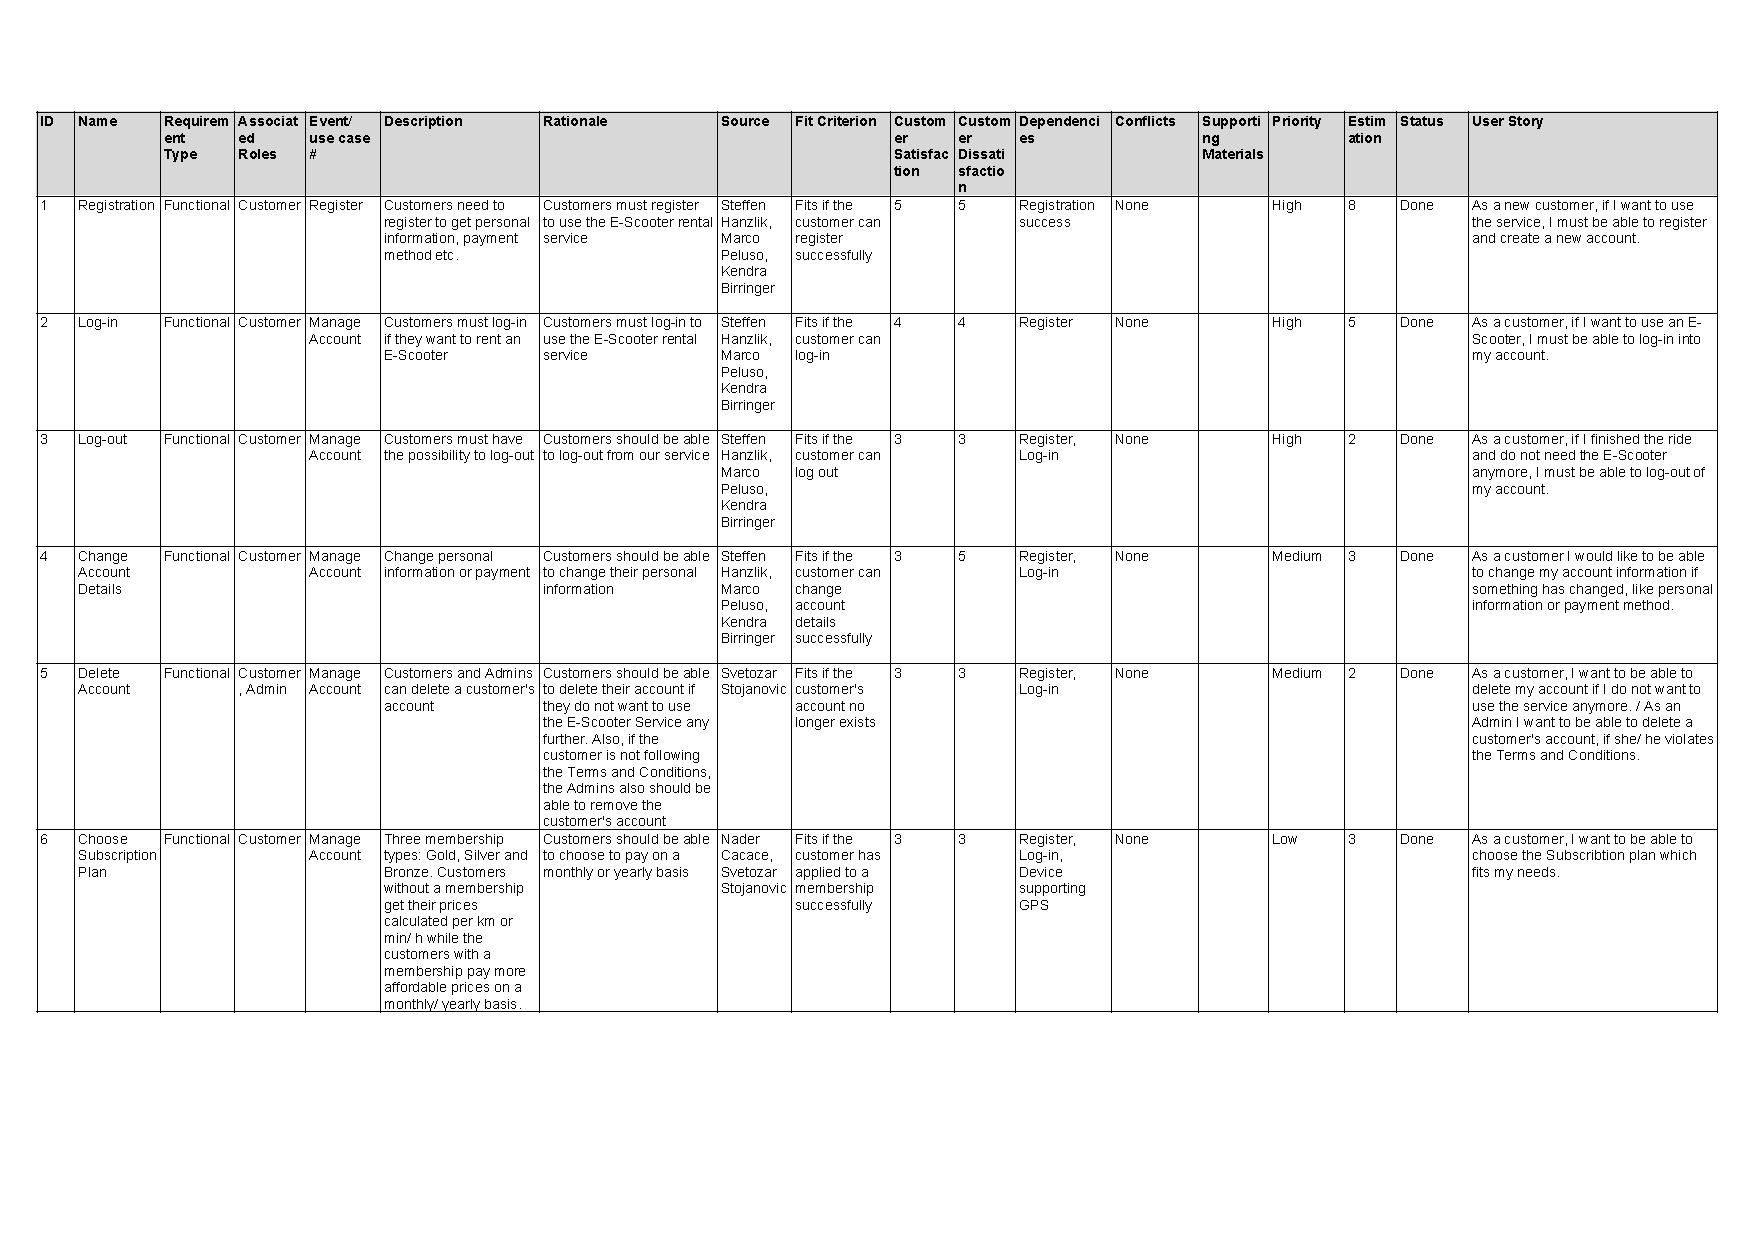
\includepdf[pages=-]{includes/pdf/project-requirements-matrix - BacklogItems.pdf}
% \end{figure}


\color{red}TODO: AUF DIE WOCHEN VERTEILEN, AUSFORMULIEREN, BEGRÜNDEN WIESO DIESE MODDELIIERT WURDEN UND DAZU SCHREIBEN WER DARAN GEARBEITET HAT UND WELCHE PROBLEME ES GAB UND WIE SIE GELÖST WURDEN UND WIESO SIE AUF DIESE ART UND WEISE SIE GELÖST WURDEN!!!
\begin{itemize}
\item Activity Diagrams:
  \item Check-in E-Scooter
  \item Check-out E-Scooter
  \item Give Feedback
  \item Log-in
  \item Log-out
  \item Manage Account
  \item Pay the Service
  \item Register
  \item Report problems with the Scooter
  
\item Sequence Diagrams:
  \item Check-in E-Scooter
  \item Check-out E-Scooter
  \item Add E-Scooter to System
  \item Find an E-Scooter on the Map
  \item Pay the Service
  \item Reserve an E-Scooter
  \item Regsiter
  \item Report Problems with the Scooter
  \item Wallet Management
    
\item UI Protypes: 
  \item Start Menu
  \item Scan QR Code
  \item Drving
  \item Menu Dropdown
  \item Account Management
  \item Change Account Details
  \item Payment Information
  \item Payment Methods
  \item Payment Methods: Credit/Debit Card
  \item Payment Method: Wallet
  \item Check Drive Statistics
  \item Check Spent Money
  \item Other
  \item Ask for feedback
  \item Register/ Sign Up
  \item Log-in
  \item Loading Screen
\end{itemize}
\color{black}

%==============================================================================
\section{Week One}
%==============================================================================
In the first week a few of our team members rented an E-Scooter from the company "Lime" to gain a better understanding of the process of renting an E-Scooter. That really helped us to find additional requirements for our E-Scooter rental service project. As we already mentioned before, we collected those requirements in a Google Sheets document. That way we could easily collaborate on them, even if we sometimes could not meet at the same location. We also started to talk about the requirements' estimations, satisfactions conditions, priorities, and fit criteria.

The estimation of the effort required to complete the backlog items, was difficult for our team, since we were all inexperienced in that regard. That's why we decided to play "Planning Poker", which is "[\ldots] a consensus-based estimating technique. Agile teams around the world use Planning Poker to estimate their product backlogs. Planning Poker can be used with story points, ideal days, or any other estimating unit." \cite{planning-poker} This proved to be very helpful and was also a lot of fun for our team.


We mostly spent the rest of the week with the collection of more requirements for the project.

Because finding dates for further meetings turned out to be difficult, we decided to hold our meetings weekly instead of daily and whenever there would occur any problems which needed to be discussed, via "Discord". Discord is an "All-in-one voice and text chat [\ldots] that's free, secure, and works on both your desktop and phone."\cite{discord}

\subsection{Division of Work: Week One}
\begin{table}[htbp]
\centering
\setlength{\tabcolsep}{10pt}
\begin{tabular}{|c|c|c|c|c|}
\hline
K. Birringer & N. Cacace & S. Hanzlik & M. Peluso & S. Stojanovic\\
\hline
\% & \% & \% & \% & \% \\ 
\hline
\end{tabular}
\end{table}

%==============================================================================
\section{Week Two}
%==============================================================================
Since we decided to use the agile method Scrum for analyzing the E-Scooter rental service project, the team members were assigned the following roles:

\begin{itemize}
\item Scrum Master: Kendra Birringer

As Scrum Master she was responsible for the organization of the whole team: she organized and moderated the team meetings and wrote the protocols. 

Another task was to check and correct the spelling, grammar and contents of everything that was written.

\item Development Team: Nader Cacace, Steffen Hanzlik,\\
      Svetozar Stojanovic

The Development Team was responsible for modeling all neccessary UML diagrams and sketching UI prototypes.

\item Tester: Marco Peluso

The Tester mainly reviewed, documented and accepted the resulting artifacts.
\end{itemize}

In the second week the team discussed each of the collected requirements, and we decided which of them fit and which are not necessary for the software. During this discussion we gathered more requirements.

Then we started to talk about the UML diagrams and built a first use case diagram which was too big and complex and needed some adjustments. So, the task for the Development Team was to simplify the diagram and make it clearer.

Also, we built a main structure for the documentation of the project and started writing the documentation with LaTex. 

\subsection{Division of Work: Week Two}

\begin{table}[htbp]
\centering
\setlength{\tabcolsep}{10pt}
\begin{tabular}{|c|c|c|c|c|}
\hline
K. Birringer & N. Cacace & S. Hanzlik & M. Peluso & S. Stojanovic\\
\hline
\% & \% & \% & \% & \% \\ 
\hline
\end{tabular}
\end{table}

%==============================================================================
\section{Week Three}
%===============================================================================
In week three the Development Team modified the use case diagram which was too big. They also modeled further use case diagrams which we then discussed, to find out if they needed further adjustments. At the end of this week, we finished the use case diagrams and finally added the use case documentation to each use case.

Also, after we thought about where it could be necessary, some activity and sequence diagrams were modeled.

Regarding the sequence diagrams there were some problems.
For example, the "Check-in" diagram:

We asked ourselves how to calculate the price for a ride. After some discussion we decided to let the wallet calculate the price for the ride information from the Scooter.
First, the payment also was included in this diagram, but after reconsidering, we decided that the payment also needed its own, more detailed diagram.

Considering the activity diagrams, we decided to not model a diagram for "Give feedback", because it seemed too simple.

Then we started to think about the class diagram and asked ourselves which classes we needed and which relations the different classes could have to each other and started modeling the class diagram.

Furthermore, a first UI prototype was built with the software design tool "Axure".\cite{axure}

\subsection{Division of Work: Week Three}
\begin{table}[htbp]
\centering
\setlength{\tabcolsep}{10pt}
\begin{tabular}{|c|c|c|c|c|}
\hline
K. Birringer & N. Cacace & S. Hanzlik & M. Peluso & S. Stojanovic\\
\hline
\% & \% & \% & \% & \% \\ 
\hline
\end{tabular}
\end{table}

%==============================================================================
\section{Week Four}
%===============================================================================
During week four we refined the state of the project by doing a lot of adjustments and modifications to everything we had done so far.
We updated the requirements, checked spelling and grammar, put the requirements in a proper order and checked what was still missing.

On the basis of the backlog items list we finished all UML diagrams and UI prototypes.
After we heard the lecture, in which Prof. Dr.-Ing Peter Thoma talked about UML diagrams, we  noticed, that all our activity diagrams lacked a cancelation mode. Therefore, we had to adjust all these diagrams and add a cancelation mode to them. 

We also finished most of the documentation, so that almost only the appendices needed to be added.

The goal of our team was, to finish everything until the end of this week, so that in the following week, we would be able to fully concentrate on the presentation of the project.

\subsection{Division of Work: Week Four}

\begin{table}[htbp]
\centering
\setlength{\tabcolsep}{10pt}
\begin{tabular}{|c|c|c|c|c|}
\hline
K. Birringer & N. Cacace & S. Hanzlik & M. Peluso & S. Stojanovic\\
\hline
\% & \% & \% & \% & \% \\ 
\hline
\end{tabular}
\end{table}

%==============================================================================
\section{Week Five}
%===============================================================================
In week five, we checked everything again and finished everything.
We generated the report from MagicDraw and added it to the documentation.
Also, we added all protocols from the team meetings.

Then we thought about a way, how to integrate the UI prototypes. We decided to screenshot each prototype and added them as an appendix to the documentation of the project.

Once the documentation was finished, each team member proofread it again and made any necessary improvements, corrections and additions.

Then, finally we started to talk about the presentation and started to build it.

%==============================================================================
\subsection{Division of Work: Week Five}

\begin{table}[htbp]
\centering
\setlength{\tabcolsep}{10pt}
\begin{tabular}{|c|c|c|c|c|}
\hline
K. Birringer & N. Cacace & S. Hanzlik & M. Peluso & S. Stojanovic\\
\hline
\% & \% & \% & \% & \% \\ 
\hline
\end{tabular}
\end{table}
%==============================================================================
\newpage
\section{Appendix}

\subsection{MagicDraw Report}
\color{red}TODO: INSERT MAGICDRAW REPORT HERE!\color{black}

\newpage
\subsection{UI Prototypes}
\begin{figure} [htbp]
  \begin{center}
    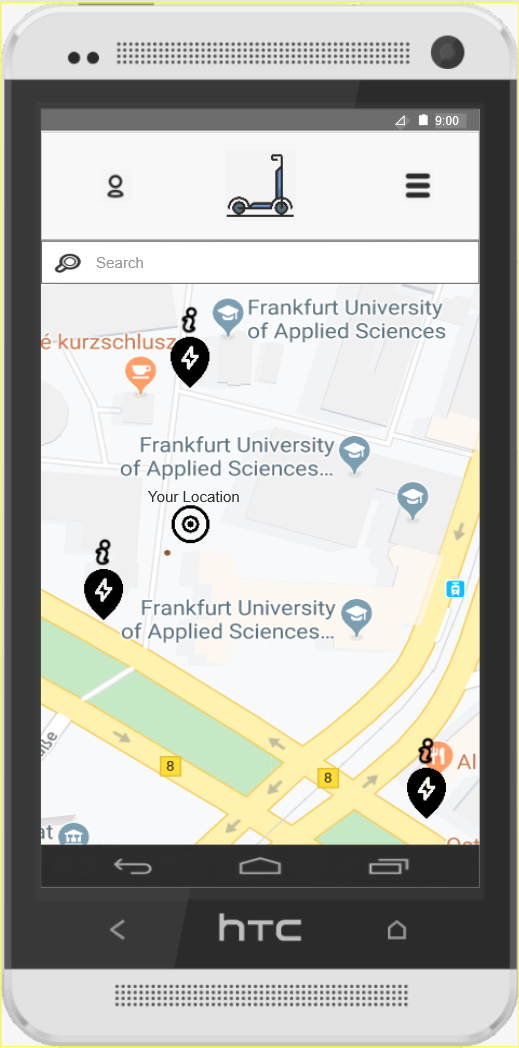
\includegraphics[scale=0.75]{images/prototypes/01-start-menu.png}
  \end{center}
  \caption{Start Menu}
\end{figure}

\begin{figure} [htbp]
  \begin{center}
    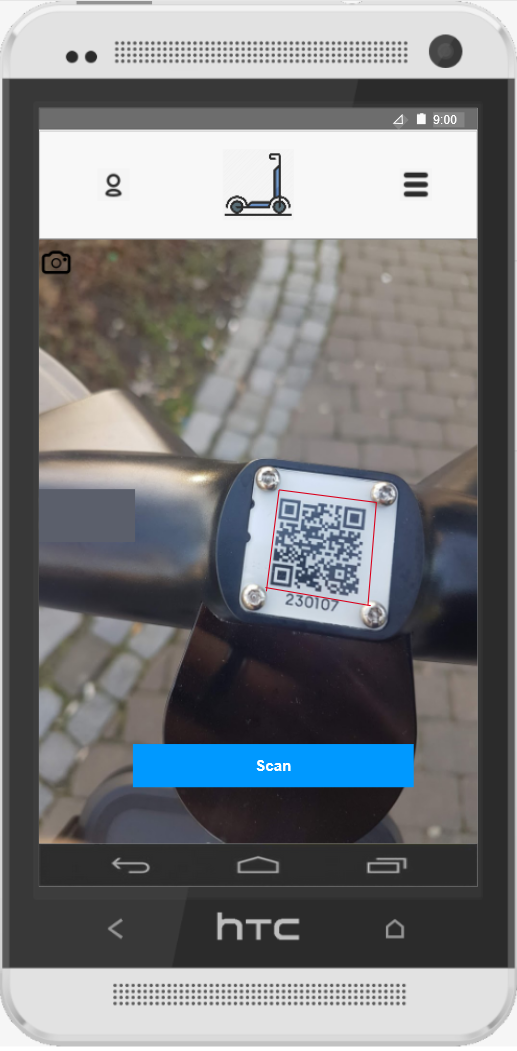
\includegraphics[scale=0.75]{images/prototypes/01-01-start-menu--scan-qr-code.png}
  \end{center}
  \caption{Start Menu $\rightarrow$ Scan QR-Code}
\end{figure}

\begin{figure} [htbp]
  \begin{center}
    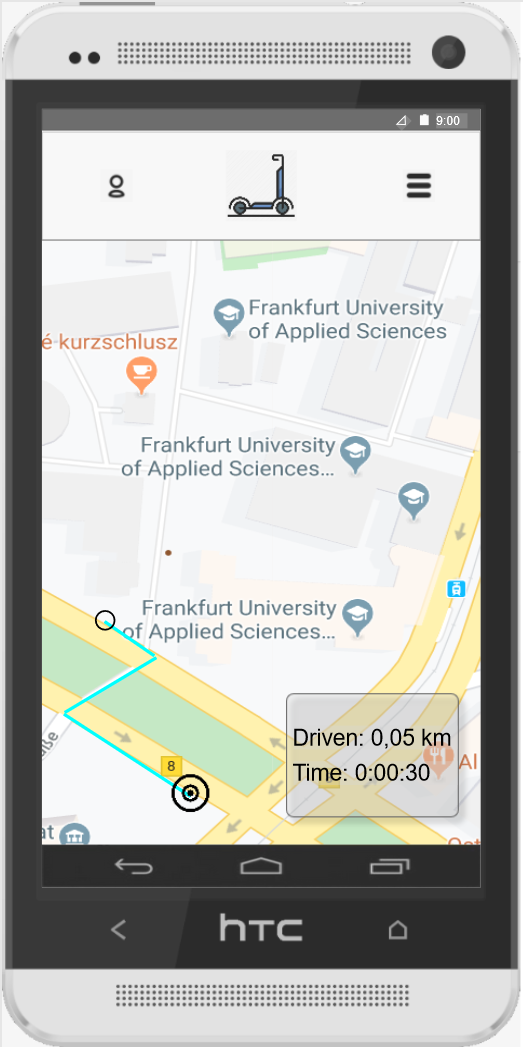
\includegraphics[scale=0.75]{images/prototypes/01-02-start-menu---driving.png}
  \end{center}
  \caption{Start Menu $\rightarrow$ Driving}
\end{figure}

\begin{figure} [htbp]
  \begin{center}
    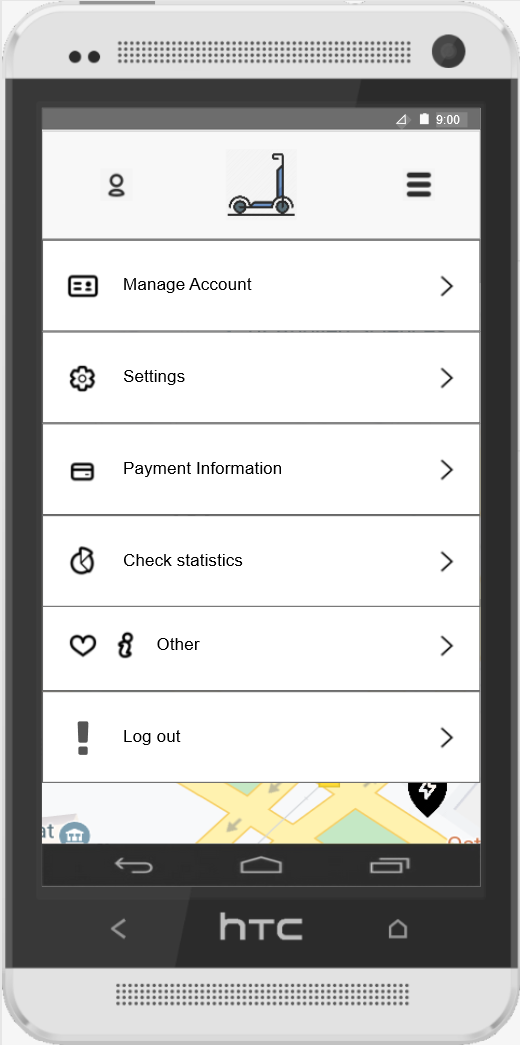
\includegraphics[scale=0.75]{images/prototypes/02-menu-dropdown.png}
  \end{center}
  \caption{Menu Dropdown}
\end{figure}

\begin{figure} [htbp]
  \begin{center}
    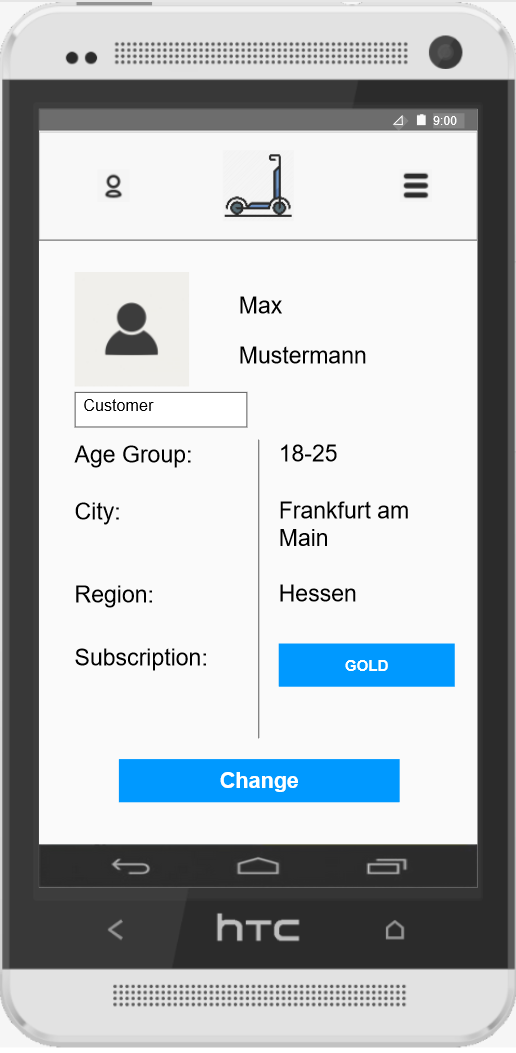
\includegraphics[scale=0.75]{images/prototypes/02-01-menu-dropdown--account-management.png}
  \end{center}
  \caption{Menu Dropdown $\rightarrow$ Account Management}
\end{figure}

\begin{figure} [htbp]
  \begin{center}
    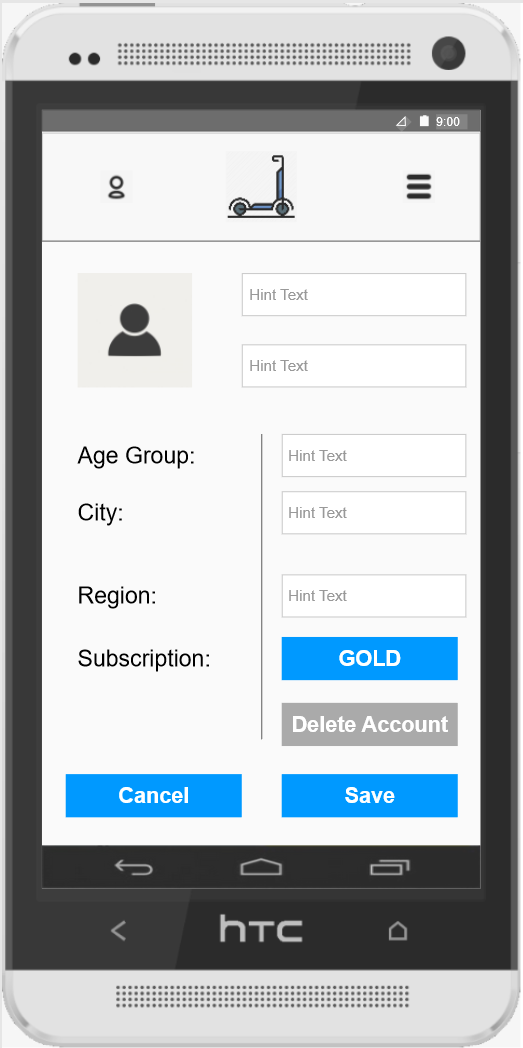
\includegraphics[scale=0.75]{images/prototypes/02-01-01-menu-dropdown--account-management--change-account-details.png}
  \end{center}
  \caption{Menu Dropdown $\rightarrow$ Account Management $\rightarrow$ Change Account Details}
\end{figure}

\begin{figure} [htbp]
  \begin{center}
    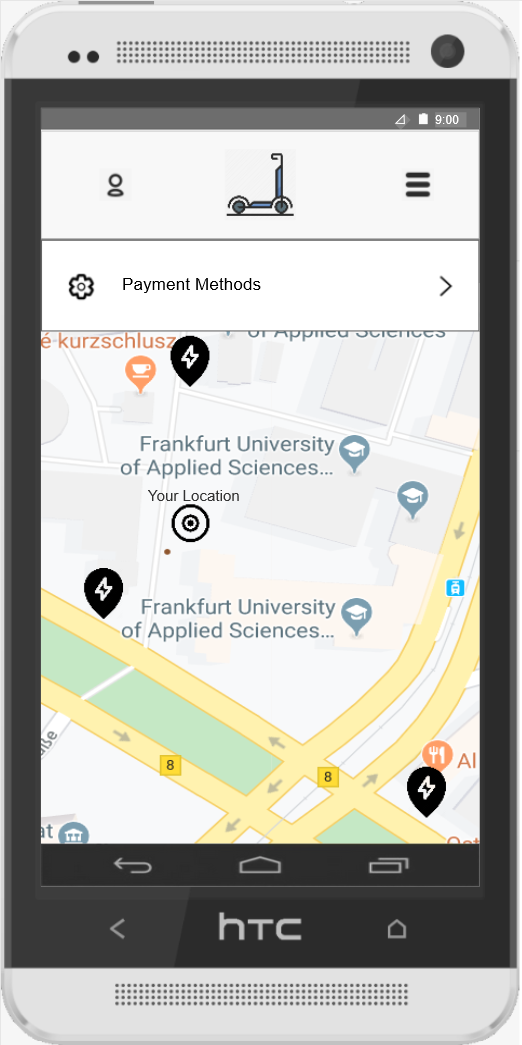
\includegraphics[scale=0.75]{images/prototypes/02-02-menu-dropdown--payment-information.png}
  \end{center}
  \caption{Menu Dropdown $\rightarrow$ Payment Information}
\end{figure}

\begin{figure} [htbp]
  \begin{center}
    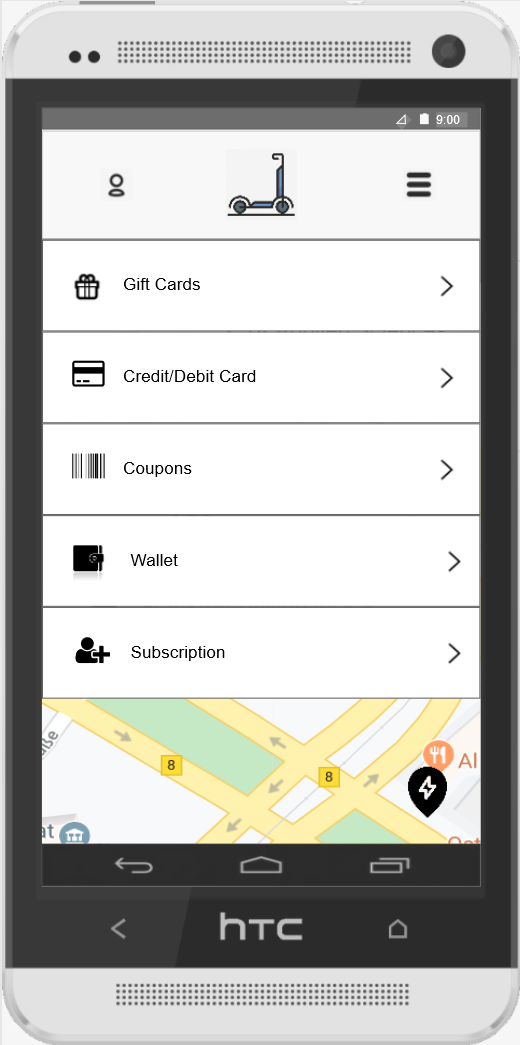
\includegraphics[scale=0.75]{images/prototypes/02-02-01-menu-dropdown--payment-information--payment-methods.png}
  \end{center}
  \caption{Menu Dropdown $\rightarrow$ Payment Information $\rightarrow$ Payment Methods}
\end{figure}

\begin{figure} [htbp]
  \begin{center}
    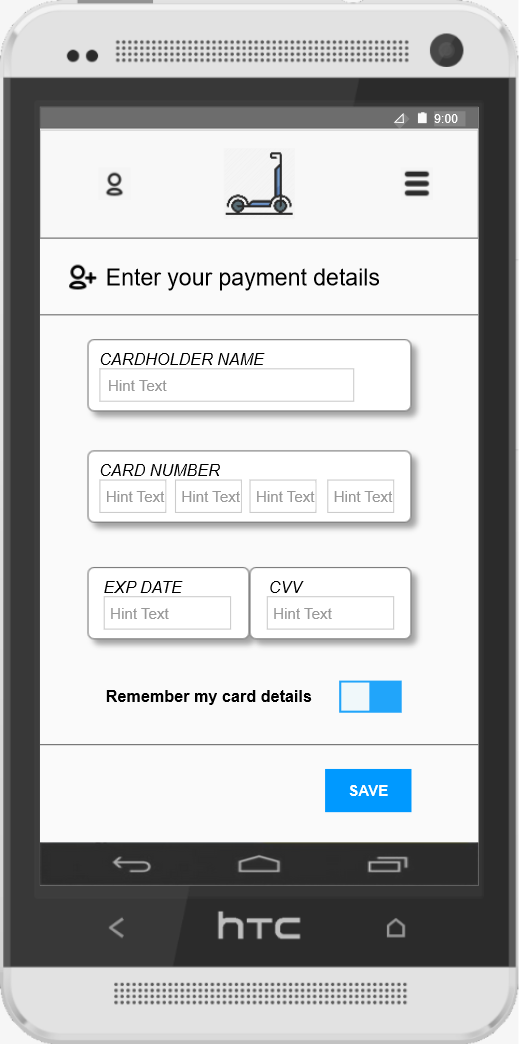
\includegraphics[scale=0.75]{images/prototypes/02-02-01-01-menu-dropdown--payment-information--payment-methods--credit-debit-card-info.png}
  \end{center}
  \caption{Menu Dropdown $\rightarrow$ Payment Information $\rightarrow$ Payment Methods $\rightarrow$ Credit/Debit Card}
\end{figure}

\begin{figure} [htbp]
  \begin{center}
    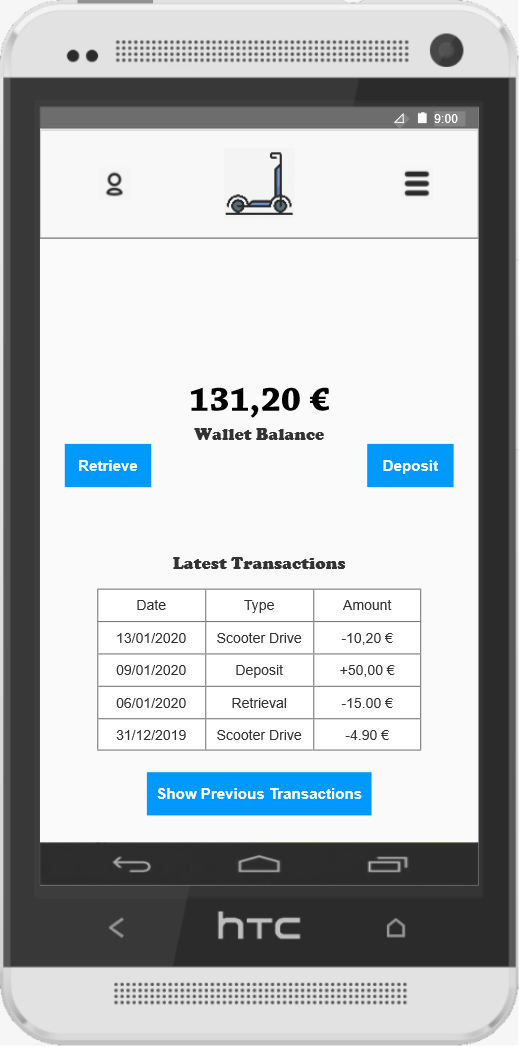
\includegraphics[scale=0.75]{images/prototypes/02-02-01-02-menu-dropdown--payment-information--payment-methods--wallet.png}
  \end{center}
  \caption{Menu Dropdown $\rightarrow$ Payment Information $\rightarrow$ Payment Methods $\rightarrow$ Wallet}
\end{figure}

\begin{figure} [htbp]
  \begin{center}
    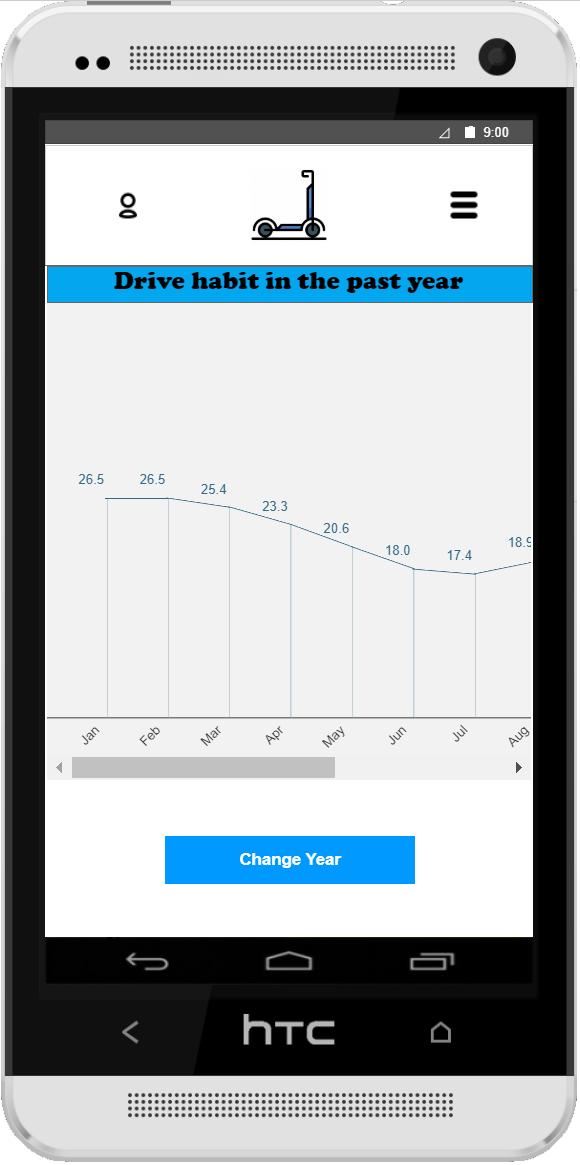
\includegraphics[scale=0.75]{images/prototypes/02-03-menu-dropdown--check-drive-statistics.png}
  \end{center}
  \caption{Menu Dropdown $\rightarrow$ Check Drive Statistics}
\end{figure}

\begin{figure} [htbp]
  \begin{center}
    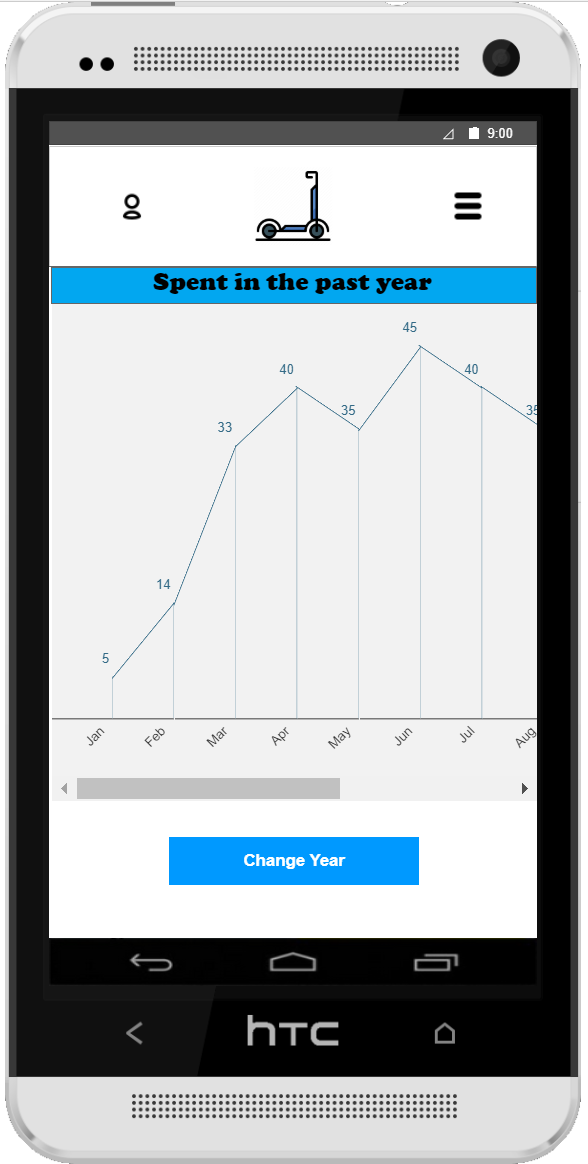
\includegraphics[scale=0.75]{images/prototypes/02-04-menu-dropdown--check-spent-money.png}
  \end{center}
  \caption{Menu Dropdown $\rightarrow$ Check Spent Money}
\end{figure}

\begin{figure} [htbp]
  \begin{center}
    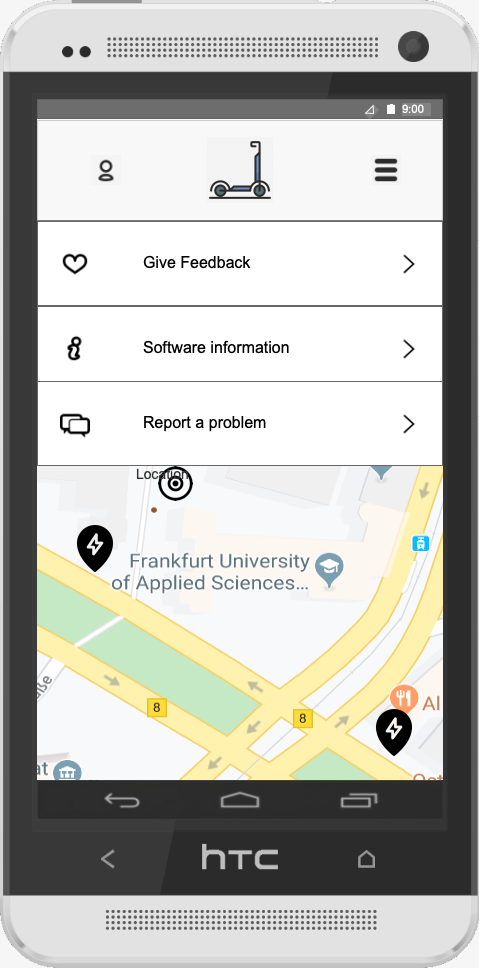
\includegraphics[scale=0.45]{images/prototypes/02-05-menu-dropdown--other.png}
  \end{center}
  \caption{Menu Dropdown $\rightarrow$ Other}
\end{figure}

\begin{figure} [htbp]
  \begin{center}
    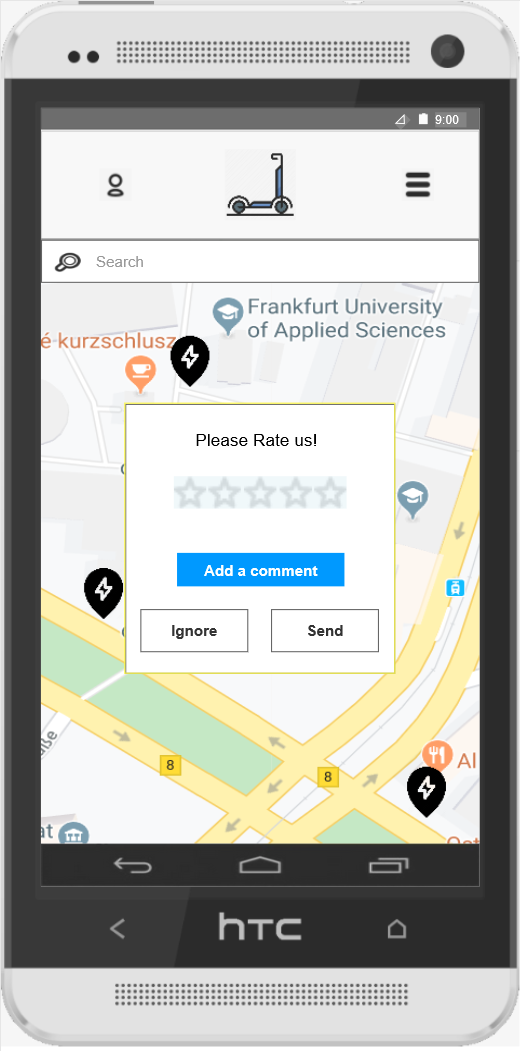
\includegraphics[scale=0.75]{images/prototypes/03-ask-for-feedback.png}
  \end{center}
  \caption{Ask for Feedback}
\end{figure}

\begin{figure} [htbp]
  \begin{center}
    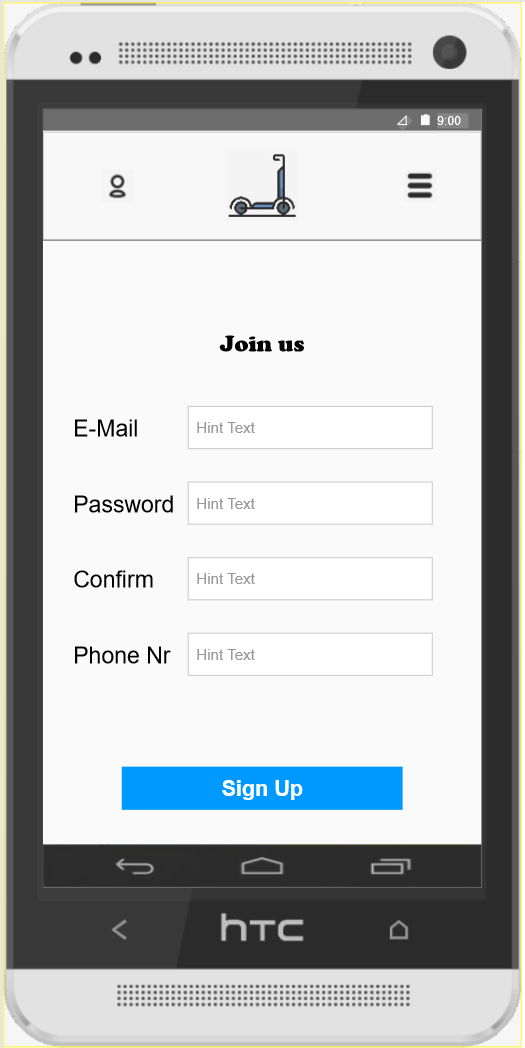
\includegraphics[scale=0.75]{images/prototypes/04-register-sign-up.png}
  \end{center}
  \caption{Register/Sign Up}
\end{figure}

\begin{figure} [htbp]
  \begin{center}
    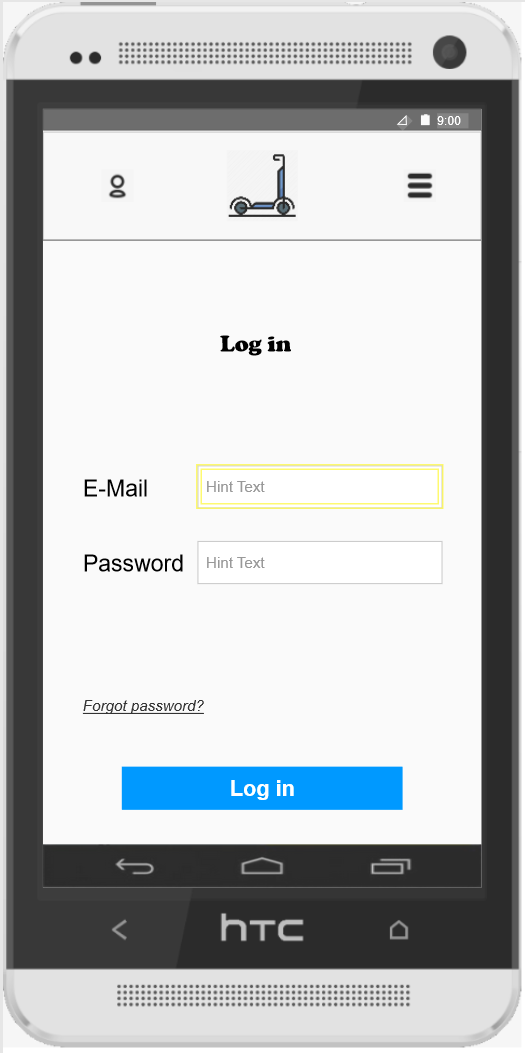
\includegraphics[scale=0.75]{images/prototypes/05-log-in.png}
  \end{center}
  \caption{Log in}
\end{figure}

\begin{figure} [htbp]
  \begin{center}
    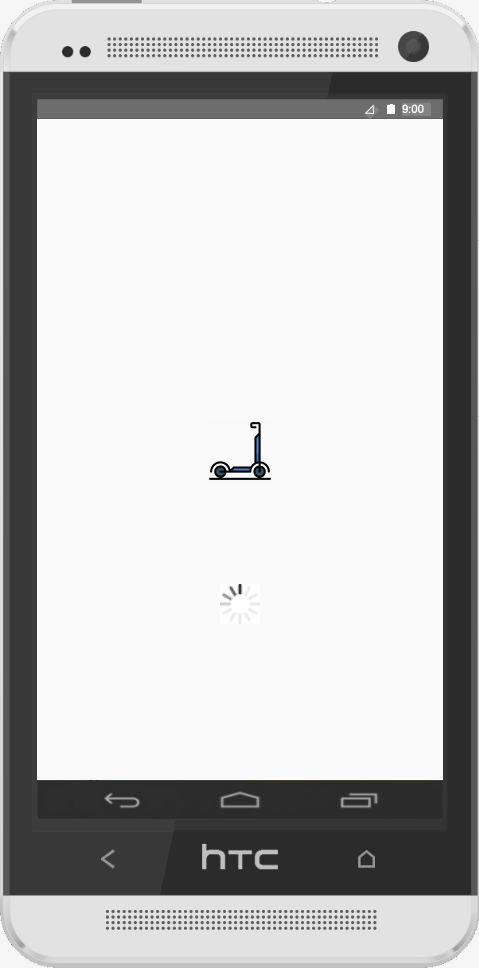
\includegraphics[scale=0.75]{images/prototypes/06-loading-screen.png}
  \end{center}
  \caption{Loading Screen}
\end{figure}

\newpage
\subsection{Meeting Protocols}
\color{red}TODO: INSERT PROTOCOLS HERE! \color{black}

%==============================================================================
\newpage
\listoffigures


%==============================================================================
\newpage
\begin{thebibliography}{}

\bibitem{scrum}
https://www.scrum.org/resources/what-is-scrum

\bibitem{uml}
https://www.omg.org/spec/UML/

\bibitem{magicdraw}
https://www.nomagic.com/products/magicdraw

\bibitem{axure}
https://www.axure.com/

\bibitem{thoma}
Prof. Dr.-Ing Peter Thoma \emph{05 Software Engineering Analysis (Software Models and UML)}

\bibitem{scrumguide}
https://www.scrumguides.org/scrum-guide.html

\bibitem{thoma1}
Prof. Dr.-Ing Peter Thoma \emph{02-3 Software Engineering Analysis (Scrum)}

\bibitem{volere}
http://www11.informatik.uni-erlangen.de/Lehre/SS2015/PR-SWE/Material/volere-template.pdf

 \bibitem{planning-poker}
https://www.mountaingoatsoftware.com/agile/planning-poker

\bibitem{discord}
https://discordapp.com/

\end{thebibliography}
%==============================================================================

\end{document}
